\documentclass{article}

\usepackage[francais]{babel}
\usepackage[T1]{fontenc}
\usepackage{fancyhdr}       % header & footer
\usepackage{moreverb}       % verbatim with tab

\usepackage{wrapfig}
\usepackage{graphicx}
\usepackage{geometry}
\geometry{hmargin=2.5cm}
\usepackage{amsmath}
\usepackage{siunitx}

\usepackage{graphicx}
\usepackage{subcaption}
\usepackage{float}
\usepackage{hyperref}
\usepackage{setspace}
\usepackage{xcolor}
\usepackage{pdfpages}
\usepackage{enumitem}
\usepackage{lscape}

\title{Réseaux industriels}
\date{2020}
\author{Laura Bin}

\begin{document}
    \pagenumbering{arabic}

    \pagestyle{fancy}
    \renewcommand\headrulewidth{1pt}
    \fancyhead[L]{Laura Binacchi}
    \fancyhead[C]{Réseaux industriels}
    \fancyhead[R]{\today}

    \begin{center}
        \textbf{\LARGE Exercice sur les librairies}
    \end{center}
    \begin{enumerate}
        \item Afin de simplifier la programmation réseau, il vous est demandé de programmer une librairie de fonctions destinée aux communications TCP v4 (v6).
        \item Compiler votre libraire pour en faire une librairie dynamique (.so sous Linux)
        \item A l'aide de la libraire réalisée plus haut, refaire les clients et serveurs pour le protocole echo.
    \end{enumerate}

    \section{Réalisation de la librairie}
    \paragraph{}
    La librairie réalisée implémente les fonctions suivantes\footnote{Prototypes dans \emph{inc/tcp-util.h} et implémentation dans \emph{lib/tcp-util.c}} :
    \begin{itemize}
        \item \texttt{int client\_connect(char *url, char *service)} : initiates an active TCP connection
        \item \texttt{int server\_listen(char *service, int backlog)} : initiates a passive TCP connection
        \item \texttt{int server\_accept(int sockfd, char *out\_client\_ip)} : accepts the connection from a client
        \item \texttt{int send\_data(int sockfd, char *buffer, ssize\_t length)} : sends data to the remote host
        \item \texttt{ssize\_t receive\_data(int sockfd, char *out\_buffer, ssize\_t max\_length)} : receives data from the remote host
        \item \texttt{int expect\_data(int sockfd, char *out\_buffer, ssize\_t length)} : expects a given amount of data from the remote host
        \item \texttt{void disconnect(int sockfd)} : closes the socket
    \end{itemize}

    \section{Compilation en librairie dynamique et liens symboliques}
    \paragraph{}
    La librairie est compilée en version 1.0 au moyen de la commande suivante\footnote{Makefile, ligne 30} :
    \begin{verbatimtab}
        cc -g -Wall -Wpedantic -Wextra -Iinc -Wl,-soname,libtcp.so.1
            -shared -fPIC -o lib/libtcp.so.1.0 lib/tcp-util.c
    \end{verbatimtab}

    \begin{description}
        \item[\texttt{cc}] compilateur utilisé
        \item[\texttt{-g}] debug
        \item[\texttt{-Wall -Wpedantic -Wextra}] warnings supplémentaires à la compilation
        \item[\texttt{-Iinc}] ajout du répertoire \emph{inc} au path des include (les fichiers présents dans le répertoire \emph{inc} peuvent être inclus par \texttt{"file.h"} au lieu de \texttt{"inc/file.h"})
        \item[\texttt{-Wl,-soname,libtcp.so.1}] les projets utilisant cette version (1.0) devront se référer à sa version majeure uniquement
        \item[\texttt{-shared}] compilation dynamique de la librairie
        \item[\texttt{-fPIC}] offsets relatifs (compilation en Position Independent Code)
        \item[\texttt{-o lib/libtcp.so.1.0}] output de la compilation
        \item[\texttt{lib/tcp-util.c}] fichier compilé
    \end{description}

    \newpage
    \paragraph{}
    La commande ldconfig me permet de créer le lien symbolique de la version 1 de ma librairie (.so.1) vers la version 1.0 (.so.1.0)\footnote{Makefile, ligne 26} :
    \begin{verbatimtab}
        ldconfig -r lib -n .
    \end{verbatimtab}

    \paragraph{}
    Je crée un lien symbolique de la librairie (.so) vers la version 1 (.so.1) avec la commande suivante\footnote{Makefile, ligne 22} :
    \begin{verbatimtab}
        ln -sf libtcp.so.1 lib/libtcp.so
    \end{verbatimtab}
    
    \section{Compilation des clients et serveurs echo avec la librairie dynamique}
    \paragraph{}
    Je compile les fichiers source en utilisant la librairie dynamique \emph{libtcp.so} avec les commandes suivantes, respectivement pour \emph{echo-client.c} et \emph{echo-server.c}\footnote{Makefile, ligne 18} :
    \begin{verbatimtab}
        cc -g -Wall -Wpedantic -Wextra -Iinc -Llib -Wl,-rpath='\$ORIGIN/lib'
            -o echo-client src/echo-client.c lib/libtcp.so
        cc -g -Wall -Wpedantic -Wextra -Iinc -Llib -Wl,-rpath='\$ORIGIN/lib'
            -o echo-server src/echo-server.c lib/libtcp.so
    \end{verbatimtab}

    \begin{description}
        \item[\texttt{-Llib}] spécifie où trouver ma librairie au moment de la compilation (dans le répertoire \emph{lib})
        \item[\texttt{-Wl,-rpath='\$ORIGIN/lib'}] commande pour le linker (lors de l'exécution) : ma librairie ne se trouve pas dans les librairies du système mais dans le répertoire relatif \emph{lib})
        \item[\texttt{-o echo-client} et \texttt{-o echo-server}] output de la compilation (fichiers exécutables)
        \item[\texttt{src/echo-client.c} et \texttt{src/echo-server.c}] fichiers source à compiler
        \item[\texttt{lib/libtcp.so}] interprété par \texttt{gmake} à partir de \texttt{-ltcp}, fait référence à ma librairie
    \end{description}

    \newpage
    \section{Installation sur les machines virtuelles}
    \paragraph{}
    Je commence par compiler le projet sur ma machine locale avec le \emph{Makefile} (dont les commandes sont détaillées plus haut) en lançant la commande \texttt{gmake}\footnote{\texttt{gmake} est utilisé à la place de \texttt{make} car le paramètre \texttt{-ltcp} est une fonctionnalité GNU}:
    \begin{figure}[H]
        \centering
        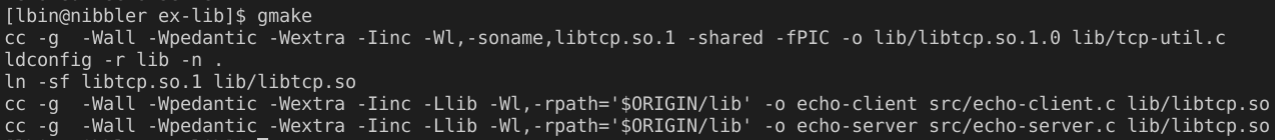
\includegraphics[width=\linewidth]{./screenshots/compilation-projet.png}
    \end{figure}

    \paragraph{}
    Les commandes prévues ont été exécutées et la racine du projet contient maintenant les exécutables \emph{echo-client} et \emph{echo-server}:
    \begin{figure}[H]
        \centering
        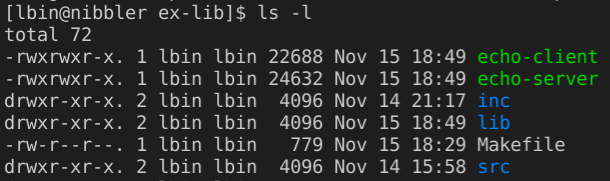
\includegraphics[width=.5\linewidth]{./screenshots/compilation-projet-exec-files.png}
    \end{figure}
    
    \paragraph{}
    Le répertoire \emph{lib} contient bien le fichier de ma librairie et les liens symboliques :
    \begin{figure}[H]
        \centering
        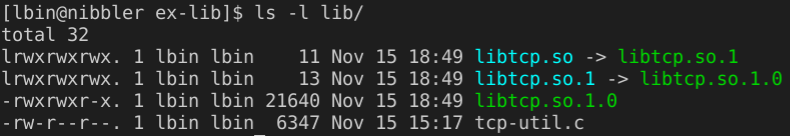
\includegraphics[width=.65\linewidth]{./screenshots/compilation-projet-lib-files.png}
    \end{figure}

    \paragraph{}
    Je copie l'exécutable du serveur et la librairie sur ma machine virtuelle :
    \begin{figure}[H]
        \centering
        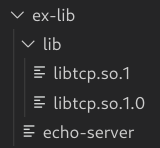
\includegraphics[width=.15\linewidth]{./screenshots/server-files.png}
    \end{figure}

    \paragraph{}
    Je recrée le lien symbolique :
    \begin{figure}[H]
        \centering
        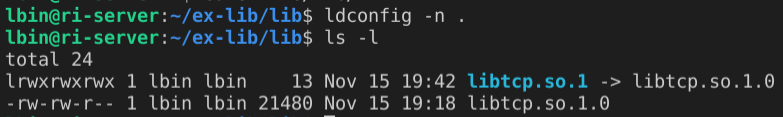
\includegraphics[width=.65\linewidth]{./screenshots/server-link.png}
    \end{figure}

    \paragraph{}
    Et je rend mon fichier \emph{echo-server} exécutable :
    \begin{figure}[H]
        \centering
        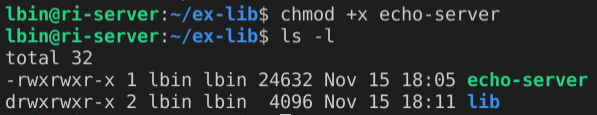
\includegraphics[width=.55\linewidth]{./screenshots/server-exec.png}
    \end{figure}

    \paragraph{}
    Je répète les mêmes opérations pour le client.

    \section{Tests}
    \subsection{Test de l'envoi d'un message simple}
    \paragraph{}
    Je lance le serveur (avec \texttt{sudo}) :
    \begin{figure}[H]
        \centering
        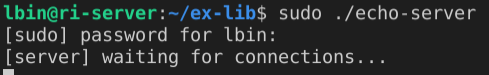
\includegraphics[width=.5\linewidth]{./screenshots/launch-server.png}
    \end{figure}

    \paragraph{}
    Je lance mon client en envoyant un message simple au serveur :
    \begin{figure}[H]
        \centering
        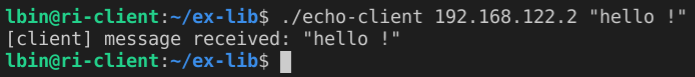
\includegraphics[width=.7\linewidth]{./screenshots/client-test-simple.png}
    \end{figure}

    \paragraph{}
    Le message a bien été renvoyé par le serveur :
    \begin{figure}[H]
        \centering
        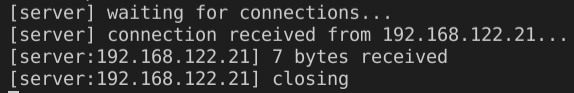
\includegraphics[width=.6\linewidth]{./screenshots/server-test-simple.png}
    \end{figure}
    
    \paragraph{}
    Après avoir renvoyé le message, le serveur ferme le socket de la connexion ouverte par le client.

    \newpage
    \subsection{Test de l'envoi d'un message de 100000 caractères}
    \paragraph{}
    Je teste l'envoi d'un message plus conséquent en augmentant la taille du buffer accepté par mon programme\footnote{La variable globale \texttt{BUF\_SIZE} est définie dans le fichier \emph{constants.h}} et en activant les messages de debug des méthodes \texttt{send\_data} et \texttt{expect\_data}\footnote{Dans le fichier \emph{tcp-util.c}} :
    % ./echo-client 127.0.0.1 "$(tr -dc '[:alnum:]' <  /dev/random | head -c 200000)"
    \begin{figure}[H]
        \centering
        
\includegraphics[width=.35\linewidth]{./screenshots/test-100000-buffer-size.png}
    \end{figure}

    \paragraph{}
    J'envoie un message contenant 100000 "1" :
    \begin{figure}[H]
        \centering
        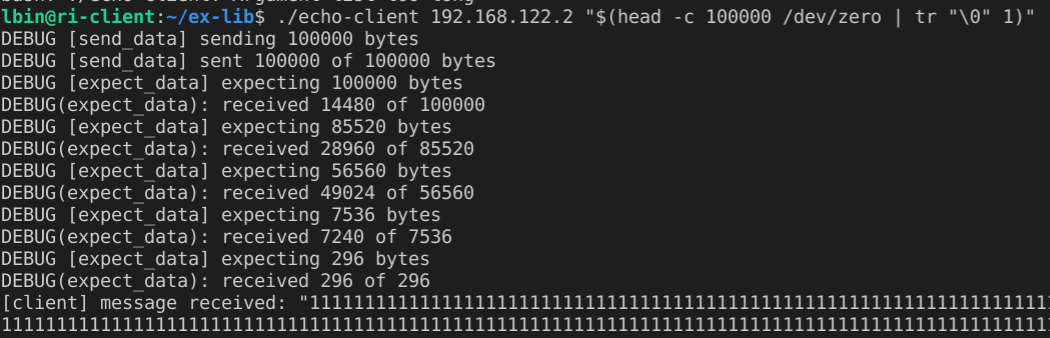
\includegraphics[width=\linewidth]{./screenshots/launch-client-100000.png}
    \end{figure}

    \paragraph{}
    Mon serveur reçoit ce message en plusieurs paquets et renvoie ces paquets :
    \begin{figure}[H]
        \centering
        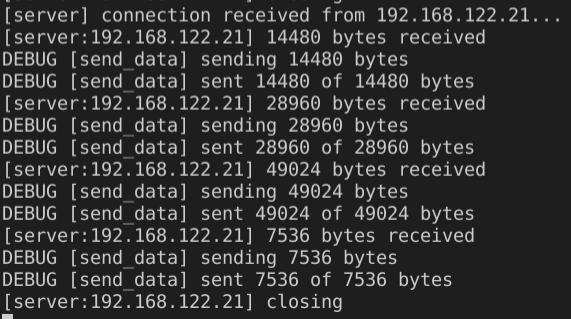
\includegraphics[width=.6\linewidth]{./screenshots/server-test-100000.png}
    \end{figure}

    \paragraph{}
    Le client, via la méthode \texttt{expect\_data}, a bien reçu les paquets renvoyés successivement par le serveur jusqu'à atteindre un message de 100000 caractères et l'afficher. En comparant les deux dernières captures d'écran, on voit bien que les tailles des paquets envoyés et reçus correspondent.

    \paragraph{}
    Enfin, ce genre de tests permet de mettre en avant l'intérêt des liens symboliques puisque pour modifier les messages de debug des méthodes de ma librairie, je n'ai du réuploader que le fichier \emph{libtcp.so.1.0} dans le répertoire \emph{lib} de mon client et de mon serveur après avoir recompilé la librairie. J'ai également dû recompiler mes exécutables pour modifier la taille du buffer. Pour simplifier cette étape, le projet pourrait être modifié en ajoutant un fichier de configuration au projet. Cela nécésitterait toutefois de modifier mes codes source avec des allocations dynamiques.
\end{document}
